\documentclass[10pt,letterpaper]{article}
\usepackage[utf8]{inputenc}
\usepackage[T1]{fontenc}
\usepackage[provide=*,spanish]{babel}
\usepackage{lmodern,geometry,amsmath,amssymb,graphicx,xcolor,microtype,multicol}
\usepackage{caption,fancyhdr,enumitem,booktabs,tabularx,array}
\usepackage[american]{circuitikz}
\usepackage{siunitx,hyperref,titlesec}
\usetikzlibrary{arrows.meta,calc}
\geometry{top=1.6cm,bottom=1.65cm,left=1.75cm,right=1.75cm,headheight=14pt}
\setlength{\columnsep}{0.65cm}
\setlength{\parindent}{0pt}
\setlength{\parskip}{0.18em}
\titlespacing*{\section}{0pt}{1.15ex plus .5ex minus .2ex}{0.55ex}
\titlespacing*{\subsection}{0pt}{0.9ex plus .35ex minus .2ex}{0.4ex}
\setlist{nosep,leftmargin=*}
\sisetup{output-decimal-marker={,},group-separator={\,},per-mode=symbol}
\captionsetup{font=small,labelfont=bf,justification=centering,skip=4pt,hypcap=false}
\definecolor{udecazul}{HTML}{003A70}
\definecolor{udecoro}{HTML}{C79A2B}
\addto\captionsspanish{\renewcommand{\tablename}{Tabla}}

% Completar los datos del grupo antes de presentar.
\newcommand{\asignatura}{Laboratorio I}
\newcommand{\laboratorio}{Propuesta de experimento}
\newcommand{\tituloinforme}{Inducción electromagnética de una espira móvil sobre un plano inclinado}
\newcommand{\autores}{\textit{[Integrantes del grupo]}}
\newcommand{\procedencia}{Departamento de Física, Universidad de Concepción, Chile}
\newcommand{\docente}{\textit{[Por completar]}}
\newcommand{\seccion}{\textit{[Sección por completar]}}
\newcommand{\fechaentrega}{\textit{[Fecha por completar]}}
\hypersetup{colorlinks=true,linkcolor=udecazul,citecolor=udecazul,urlcolor=udecazul,
 pdftitle={Inducción electromagnética con un carrito sobre plano inclinado},
 pdfauthor={Grupo de Laboratorio I}}
\pagestyle{fancy}
\fancyhf{}
\lhead{\small \laboratorio: Inducción electromagnética}
\rhead{\small \asignatura}
\cfoot{\small \thepage}
\renewcommand{\headrulewidth}{0.4pt}
\fancypagestyle{plain}{\fancyhf{}\lhead{\small \laboratorio: Inducción electromagnética}\rhead{\small \asignatura}\cfoot{\small \thepage}}

\begin{document}
\thispagestyle{empty}
\begin{center}
  \begin{minipage}{0.46\textwidth}
    \raggedright
    
\includegraphics[width=0.68\linewidth]{figuras/logo_udec.png}
  \end{minipage}
  \begin{minipage}{0.46\textwidth}
    \raggedleft
    
\includegraphics[width=0.68\linewidth]{figuras/logo_fcfm.png}
  \end{minipage}
  {\color{udecoro}\rule{0.82\textwidth}{1.2pt}\par}
  \vspace{0.10cm}
  {\Large\bfseries \asignatura\par}
  \vspace{0.12cm}
  {\large\bfseries\color{udecazul} \laboratorio\par}
  \vspace{0.10cm}
  {\Large\bfseries\color{udecazul} \tituloinforme\par}
  \vspace{0.09cm}
  {\normalsize Objetivo, modelo físico y método de medición\par}
  \vspace{0.11cm}
  {\small \autores\par}
  {\footnotesize\itshape \procedencia\par}
  \vspace{0.05cm}
  {\small Docente: \docente\par}
  {\small \seccion \quad $\vert$ \quad \fechaentrega\par}
\end{center}

\begin{abstract}
Se propone estudiar la tensión inducida en una espira conductora transportada por un carrito que desciende sobre un riel inclinado. Dos bobinas de Helmholtz alimentadas con corriente continua producen un campo magnético externo, y un osciloscopio registra la señal eléctrica durante el movimiento. La variable independiente será el ángulo del riel y la dependiente, la amplitud del voltaje inducido. El modelo combina la dinámica del plano inclinado y la ley de Faraday--Lenz, considerando que la orientación de la espira y el perfil espacial del campo influyen en la señal.
\end{abstract}

\begin{multicols}{2}
\raggedcolumns

\section{Introducción}

Una variación del flujo magnético a través de una espira conductora origina una fuerza electromotriz inducida, según la ley de Faraday--Lenz. En esta experiencia se busca producir dicha variación desplazando una espira sobre un carrito a través del campo magnético generado por un par de bobinas de Helmholtz. Al modificar la inclinación del riel cambia la rapidez del carrito y, con ello, la rapidez de variación del flujo. Se pretende contrastar esta relación mediante la amplitud de la tensión registrada con un osciloscopio.

\section{Objetivo y variables}

\textbf{Objetivo.} Estudiar cómo cambia la amplitud de la tensión inducida cuando se modifica el ángulo de inclinación del riel, manteniendo constante la distancia de liberación y, en lo posible, las condiciones magnéticas y eléctricas.

\textbf{Variable independiente:} ángulo de inclinación $\theta$ del riel.

\textbf{Variable dependiente:} amplitud máxima $U_{\mathrm{pk}}$ de la tensión inducida, medida respecto de la línea base del osciloscopio.

\textbf{Variables de control:} distancia de liberación $d$, corriente $I_H$ de Helmholtz, número de vueltas $N_e$ y dimensiones de la espira, resistencia de carga y forma de soltar el carrito. Se procurará mantener su orientación respecto del campo y una trayectoria comparable entre ensayos.

\section{Marco teórico}

\subsection{Movimiento del carrito}

Tomando un eje paralelo al riel y positivo hacia abajo, la segunda ley de Newton, al despreciar el rozamiento y el frenado electromagnético, entrega
\begin{equation}
  ma=mg\sin\theta
  \quad\Rightarrow\quad a=g\sin\theta.
  \label{eq:aceleracion}
\end{equation}
Si el carrito parte del reposo y recorre una distancia fija $d$ antes de alcanzar una zona de referencia, la cinemática de aceleración constante conduce a
\begin{equation}
  \boxed{v=\sqrt{2gd\sin\theta}.}
  \label{eq:velocidad}
\end{equation}
Esta rapidez es una predicción ideal; el rozamiento de las ruedas y otros efectos pueden disminuirla.

\subsection{Campo magnético y flujo}

Las bobinas de Helmholtz son dos bobinas circulares coaxiales de radio $R_H$, separadas una distancia $R_H$, con $N_H$ vueltas por bobina y corriente $I_H$ en el mismo sentido. En el punto central producen un campo de magnitud
\begin{equation}
 B_H(0)=\left(\frac45\right)^{3/2}
 \frac{\mu_0 N_H I_H}{R_H}.
 \label{eq:helmholtz}
\end{equation}
El campo es aproximadamente uniforme solo cerca del centro. En las regiones de entrada y salida su valor cambia gradualmente con la posición.

El flujo magnético por una vuelta de la espira se define como
\begin{equation}
 \boxed{\Phi_B=\int_S\vec B\cdot d\vec S.}
 \label{eq:flujo}
\end{equation}
Si el campo varía poco sobre el área $A$ de la espira, puede utilizarse $\Phi_B\simeq BA\cos\beta$, donde $\beta$ es el ángulo entre el campo y la \emph{normal} al plano de la espira. El movimiento induce tensión únicamente cuando cambia este flujo, no por la rapidez aislada del carrito.

\subsection{Ley de Faraday--Lenz}

Para un circuito móvil de $N_e$ vueltas que enlazan aproximadamente el mismo flujo, la fuerza electromotriz (fem) inducida cumple \cite{chi2017,serway2009}
\begin{equation}
 \boxed{\mathcal E=-N_e\frac{d\Phi_B}{dt}.}
 \label{eq:faraday}
\end{equation}
El signo negativo expresa la ley de Lenz: el sentido de la corriente inducida se opone a la variación del flujo. Puesto que el campo externo se mantiene estacionario y el flujo depende de la posición $s$ sobre el riel, la regla de la cadena permite escribir
\begin{equation}
 \boxed{\mathcal E=-N_e\frac{d\Phi_B}{ds}\,v.}
 \label{eq:faraday_movimiento}
\end{equation}
Esta expresión muestra que, para un mismo gradiente espacial de flujo, la magnitud de la fem es proporcional a la rapidez. Cuando el carrito entra y sale de una región de flujo distinto, pueden aparecer pulsos de polaridad opuesta. Cerca de una zona donde el flujo apenas cambia, la fem puede ser pequeña incluso si el carrito se mueve.

\subsection{Tensión registrada y predicción}

Se considera una espira con resistencia propia $r_e$ y una resistencia de carga $R_L$. Si la respuesta del circuito es aproximadamente resistiva y la impedancia del osciloscopio es mucho mayor que $R_L$, la tensión medida en esta última es
\begin{equation}
 V_R(t)\simeq\frac{R_L}{r_e+R_L}\,\mathcal E(t).
 \label{eq:voltaje}
\end{equation}
Para comparar ensayos se utilizará el máximo absoluto de la señal tras restar su línea base $V_0$:
\begin{equation}
 U_{\mathrm{pk}}=\max_t|V_R(t)-V_0|.
 \label{eq:pico}
\end{equation}
Si entre mediciones se mantiene aproximadamente constante el gradiente relevante de flujo y el acoplamiento geométrico, las ecuaciones \eqref{eq:velocidad} y \eqref{eq:faraday_movimiento} predicen
\begin{equation}
 \boxed{U_{\mathrm{pk}}\propto\sqrt{\sin\theta}.}
 \label{eq:hipotesis}
\end{equation}
Esta proporcionalidad es una \emph{predicción ideal}. En la disposición propuesta, el campo central es aproximadamente transversal al riel y la espira se orienta para que su normal sea casi paralela a $\vec B$. Se supone que, al variar $\theta$, la espira recorre regiones comparables del campo; los posibles cambios de trayectoria se considerarán como fuente de error experimental.

\section{Montaje y medición propuestos}

Se instalarán las bobinas de Helmholtz fijas y alimentadas con corriente continua, una a cada lado del riel. Sus planos serán verticales y su eje común horizontal, transversal al desplazamiento del carrito, que pasará por la región central sin atravesar los aros. La espira captadora se fijará verticalmente sobre el carrito, en el plano longitudinal del riel, de forma que su normal se oriente aproximadamente con el campo central. Su forma, tamaño y número de vueltas dependerán del material disponible.

\begin{center}
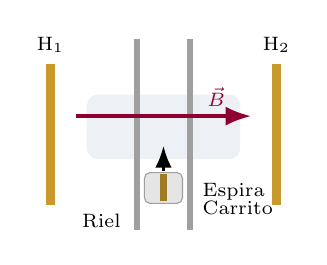
\begin{tikzpicture}[scale=0.78,>=Latex, every node/.style={font=\scriptsize}]
  % Vista superior: los planos de las bobinas son verticales.
  \fill[udecazul!7,rounded corners=4pt] (-1.25,-0.40) rectangle (1.25,0.65);
  \draw[gray!75,line width=2.0pt] (-0.43,-1.55)--(-0.43,1.55);
  \draw[gray!75,line width=2.0pt] (0.43,-1.55)--(0.43,1.55);
  \draw[udecoro,line width=3.0pt] (-1.84,-1.15)--(-1.84,1.15);
  \draw[udecoro,line width=3.0pt] (1.84,-1.15)--(1.84,1.15);
  \node[above] at (-1.84,1.17) {H$_1$};
  \node[above] at (1.84,1.17) {H$_2$};
  \draw[->,line width=1.4pt,purple!75!black] (-1.43,0.30)--(1.43,0.30);
  \node[above,purple!75!black] at (0.86,0.30) {$\vec B$};
  \draw[fill=gray!20,draw=gray!75,rounded corners=2pt] (-0.31,-1.12) rectangle (0.31,-0.62);
  \draw[line width=2.2pt,udecoro!80!black] (0,-1.08)--(0,-0.65);
  \draw[->,line width=1.1pt] (0,-0.59)--(0,-0.18);
  \node[anchor=west] at (0.48,-0.93) {Espira};
  \node[anchor=west] at (0.48,-1.19) {Carrito};
  \node[anchor=east] at (-0.54,-1.41) {Riel};
\end{tikzpicture}
\captionof{figure}{Vista superior del montaje propuesto (no a escala).}
\label{fig:montaje}
\end{center}

Para variar $\theta$, se elevará un extremo del riel mediante un soporte, manteniendo apoyado el otro. En cada ensayo se conservará la distancia $d$ de liberación respecto de una referencia cercana al centro magnético; el carrito se soltará sin impulso inicial. Se procurará que la espira cruce regiones comparables del campo. Los cambios de altura al inclinar el riel se considerarán como posible fuente de error.

\begin{center}
\begin{circuitikz}[american,scale=0.83,transform shape]
  \draw (0,0) to[V,l_=$\mathcal E(t)$] (0,2.1)
   to[R,l=$r_e$] (1.85,2.1)
   to[R,l=$R_L$] (4.05,2.1)
   -- (4.05,0) -- (0,0);
  \draw (1.85,2.1) -- (1.85,3.0) -- (2.67,3.0);
  \node[draw,circle,minimum size=0.62cm,inner sep=0pt] (scope) at (3.0,3.0) {$V$};
  \draw (scope.east) -- (4.05,3.0) -- (4.05,2.1);
  \node[font=\scriptsize,anchor=south] at (3.0,3.37) {Osciloscopio};
\end{circuitikz}
\captionof{figure}{Circuito equivalente propuesto: la fem de la espira móvil se registra como voltaje en $R_L$.}
\label{fig:circuito}
\end{center}

El osciloscopio se conectará en paralelo con $R_L$. Para cada ángulo se registrarán la línea base, los máximos de ambas polaridades y la duración de los pulsos, con varias repeticiones y alimentación de Helmholtz constante. Si se emplea el Hameg HM203-7, será conveniente filmar la traza, ya que no almacena los pulsos. Los cables no deberán frenar el carrito ni generar señales parásitas apreciables.

\textbf{Contraste experimental.} Se graficará $U_{\mathrm{pk}}$ frente a $\sqrt{\sin\theta}$, considerando la dispersión e incertidumbres. Si se dispone de una medida independiente de rapidez, también se contrastará $U_{\mathrm{pk}}$ con $v$.

\textbf{Condición previa.} Se comprobará que la normal de la espira esté aproximadamente orientada en la dirección del campo central y que la señal inducida resulte detectable. Si el campo es paralelo al plano de la espira, el flujo y la señal pueden ser muy pequeños.

\begin{thebibliography}{9}
\bibitem{chi2017} R. Chi Durán, \emph{Problemas propuestos y resueltos de electromagnetismo}, versión marzo de 2017, cap.~15 (ley de Faraday--Lenz).
\bibitem{serway2009} R. A. Serway y J. W. Jewett, Jr., \emph{Física para ciencias e ingeniería con física moderna}, vol.~2, 7.\textsuperscript{a} ed., Cengage Learning, 2009, caps.~30--31.
\end{thebibliography}

\end{multicols}
\end{document}
